\newcommand{\scaler}{0.6}
\newcommand{\plytawidth}{10cm*\scaler}
\newcommand{\plytalength}{2.5cm*\scaler}
\newcommand{\plytaheight}{5cm*\scaler}
\newcommand{\railcoor}{2cm*\scaler}
\newcommand{\railwidth}{0.4cm*\scaler}
\newcommand{\railheight}{0.6cm*\scaler}
\newcommand{\xots}{0.5cm*\scaler}
\newcommand{\eots}{0.15cm*\scaler}
\newcommand{\diagox}{0.1cm*\scaler}
\newcommand{\pressx}{1cm*\scaler}
\newcommand{\pressy}{0.5cm*\scaler}
\newcommand{\diagx}{0.15cm*\scaler}
\newcommand{\diagy}{0.15cm*\scaler}
\newcommand{\stalplytax}{0.2cm*\scaler}
\newcommand{\stalplytay}{1.5cm*\scaler}
\newcommand{\arrowlength}{0.6cm*\scaler}
\newcommand{\newgeom}{5cm*\scaler}
\newcommand{\newgeomx}{8cm*\scaler}
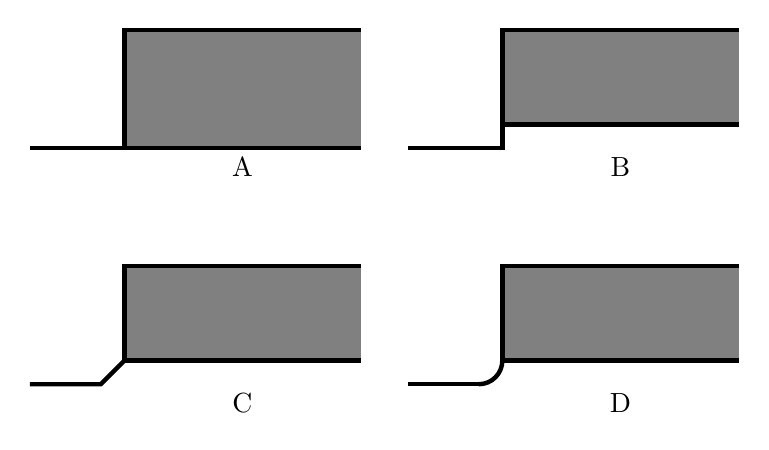
\begin{tikzpicture}
  \coordinate (A) at (0, 0);
  \coordinate (B) at (0, \plytalength);
  \coordinate (C) at (\plytawidth/2, 0);
  \coordinate (D) at (\plytawidth/2, \plytalength);
  \coordinate (E) at (-\railcoor, 0);
  \coordinate (F) at (\plytawidth/4, 0);
   
  \draw [ultra thick, fill=gray] (C) -- (A) -- (B) -- (D);
  \draw [ultra thick] (E) -- (A);
  \node [below] at (F) {A};
  
  \coordinate (A1) at (\newgeomx, \pressy);
  \coordinate (B1) at (\newgeomx, \plytalength);
  \coordinate (C1) at (\newgeomx + \plytawidth/2, \pressy);
  \coordinate (D1) at (\newgeomx + \plytawidth/2, \plytalength);
  \coordinate (E1) at (\newgeomx - \railcoor, 0);
  \coordinate (F1) at (\newgeomx + \plytawidth/4, 0);
  \coordinate (H1) at (\newgeomx,  0);
  \coordinate (G1) at (\newgeomx + \plytawidth, 0);
   
  \draw [ultra thick, fill=gray] (C1) -- (A1) -- (B1) -- (D1);
  \draw [ultra thick] (E1) -- (H1) -- (A1);
  \node [below] at (F1) {B};
  
  \coordinate (A2) at (0, \pressy - \newgeom);
  \coordinate (B2) at (0, \plytalength - \newgeom);
  \coordinate (C2) at (\plytawidth/2, \pressy - \newgeom);
  \coordinate (D2) at (\plytawidth/2, \plytalength - \newgeom);
  \coordinate (E2) at (-\railcoor,  - \newgeom);
  \coordinate (F2) at (\plytawidth/4,  -\newgeom);
  \coordinate (H2) at (- \pressy,  - \newgeom);
  \coordinate (G2) at (\plytawidth + \pressy,  - \newgeom);
   
  \draw [ultra thick, fill=gray] (C2) -- (A2) -- (B2) -- (D2);
  \draw [ultra thick] (E2) -- (H2) -- (A2);
  \node [below] at (F2) {C};
  
  \coordinate (A3) at (\newgeomx, \pressy - \newgeom);
  \coordinate (B3) at (\newgeomx, \plytalength - \newgeom);
  \coordinate (C3) at (\newgeomx + \plytawidth/2, \pressy - \newgeom);
  \coordinate (D3) at (\newgeomx + \plytawidth/2, \plytalength - \newgeom);
  \coordinate (E3) at (\newgeomx-\railcoor,  -\newgeom);
  \coordinate (F3) at (\newgeomx + \plytawidth/4, -\newgeom);
  \coordinate (H3) at (\newgeomx - \pressy,  -\newgeom);
  \coordinate (G3) at (\newgeomx + \plytawidth + \pressy,  -\newgeom);
  \coordinate (T3) at (\newgeomx - \pressy,  -\newgeom);
  \coordinate (Y3) at (\newgeomx + \plytawidth,  -\newgeom + \pressy);
   
  \draw [ultra thick, fill=gray] (C3) -- (A3) -- (B3) -- (D3);
  \draw [ultra thick] (E3) -- (H3);
  \draw [ultra thick] (T3) arc [radius=\pressy, start angle=270, end angle= 360];
  \node [below] at (F3) {D};

 
\end{tikzpicture}